\section{Development process}

In the initial stages of software development, there was a lack of reference models, leading to a straightforward "code and fix" approach. 
In response to the previously mentioned software crisis, the necessity for a structured model became evident.
The first comprehensive model introduced was the "waterfall" model, characterized by the following fundamental requirements:
\begin{enumerate}
    \item Identification of distinct phases and associated activities.
    \item Enforcement of a linear progression, with no backtracking between phases.
    \item Standardization of outputs generated at each phase.
    \item Viewing software development as akin to a manufacturing process.
\end{enumerate}
Following the advent of the waterfall model, numerous more flexible methodologies emerged, including iterative models, the agile movement, and DevOps, which aimed to offer more adaptable approaches to software development.
\begin{figure}[H]
    \centering
    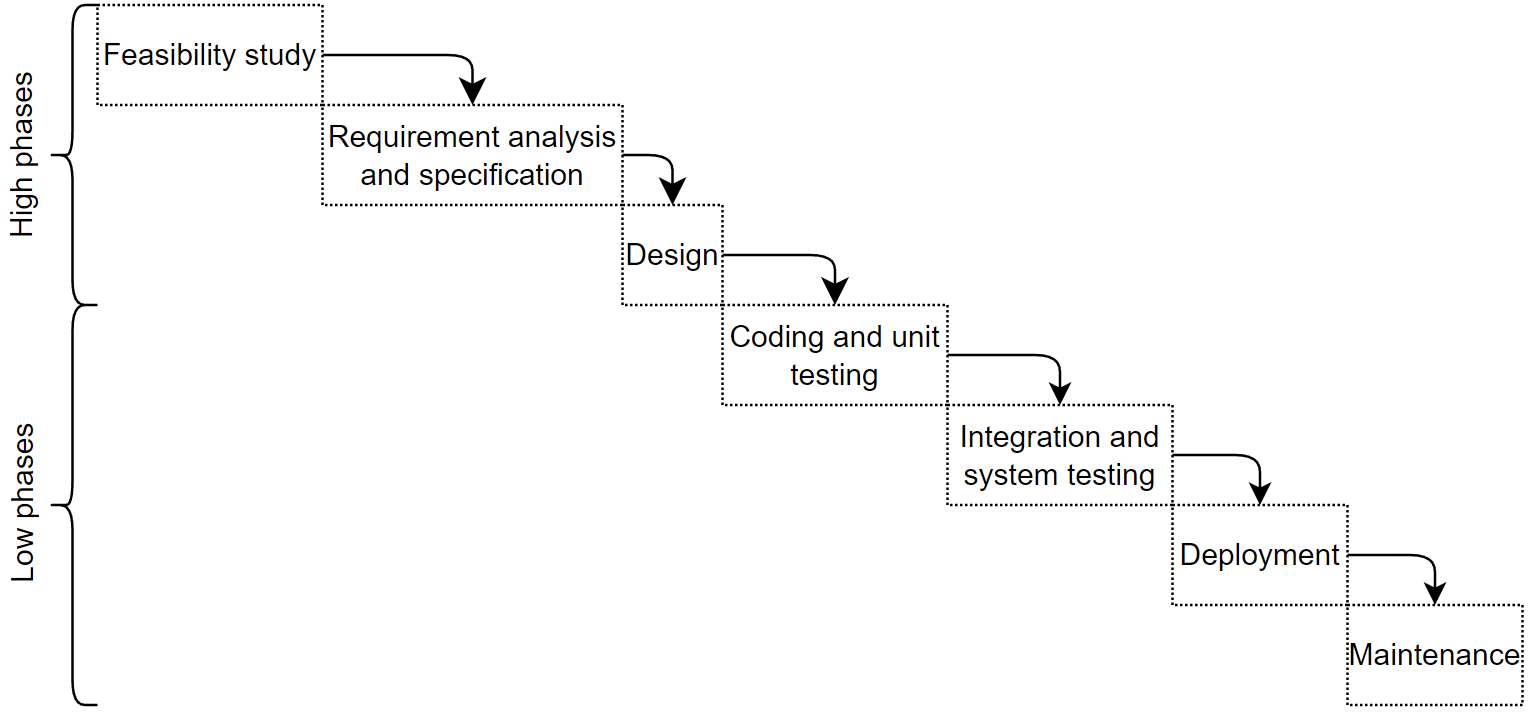
\includegraphics[width=0.75\linewidth]{images/waterfall.png}
    \caption{Waterfall process model}
\end{figure}
The key phases depicted in the image encompass the following:
\begin{enumerate}
    \item \textit{Feasibility study and project estimation}: this stage determines whether the project should commence, exploring possible alternatives and necessary resources. 
        It yields a "feasibility study document" comprising an initial problem description, scenarios outlining potential solutions, and cost and schedule estimates for various options.
    \item \textit{Requirement analysis and specification}: in this phase, the domain in which the application operates is meticulously analyzed. 
        Requirements are identified, and software specifications are derived, leading to the creation of a "requirement analysis and specification document". 
    \item \textit{Design}: this step outlines the software architecture, defining components, their relationships, and interactions. 
        The objective is to facilitate concurrent development and allocate responsibilities. 
        It culminates in the production of a "design document". 
    \item \textit{Coding and unit test}: each module is implemented and rigorously tested. 
        Additional quality assurance measures, such as inspections, may be employed. 
        Programs are accompanied by their respective documentation.
    \item \textit{Integration and system test}: modules are integrated into systems, and the integrated systems undergo testing. 
        This phase, as well as the preceding one, can be integrated into an incremental implementation scheme.
    \item \textit{Deployment}.
    \item \textit{Maintenance}: the maintenance phase comprises various aspects, including:
        \begin{itemize}
            \item \textit{Corrective}: addressing and rectifying identified faults or defects.
            \item \textit{Adaptive}: adapting the software to changes in its environment.
            \item \textit{Perfective}: accommodating new or modified user requirements.
            \item \textit{Preventive}: involving activities aimed at enhancing the system's maintainability.
        \end{itemize}
\end{enumerate}
\begin{figure}[H]
    \centering
    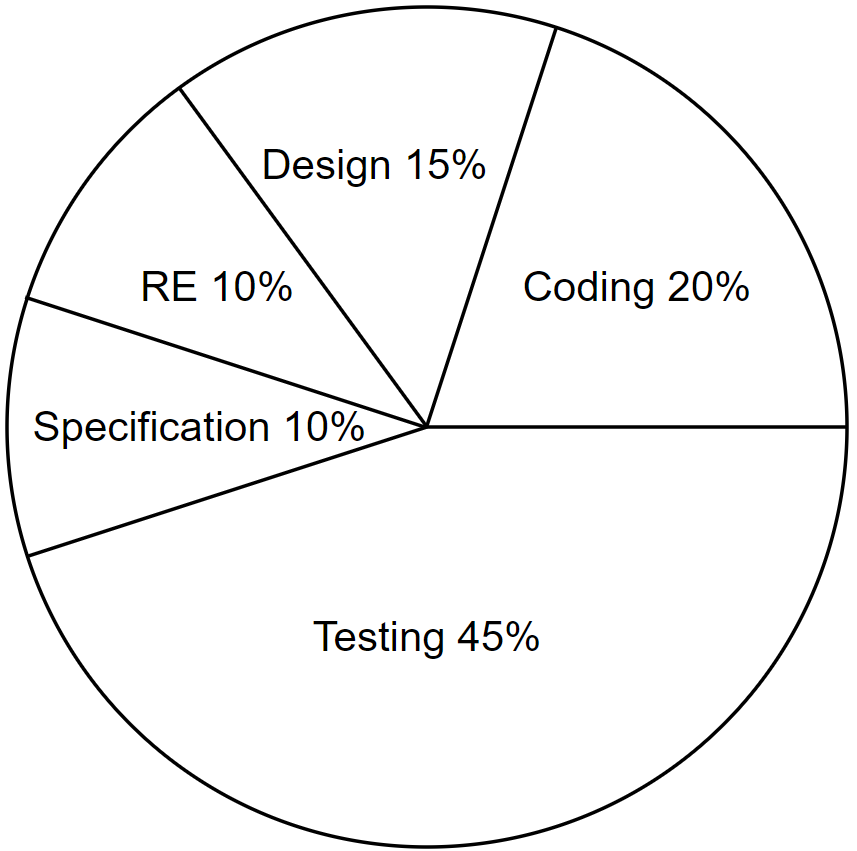
\includegraphics[width=0.35\linewidth]{images/effort.png}
    \caption{Effort in each phase}
\end{figure}

The primary challenges associated with software evolution include:
\begin{itemize}
    \item It is seldom anticipated and strategically planned.
    \item Software is highly amenable to change, with modifications often directly affecting the code, leading to inconsistencies in project documentation.
\end{itemize}
Effectively addressing software evolution necessitates the implementation of sound engineering practices, comprising two key steps: first, modifying the design, and then making corresponding adjustments in the implementation, ensuring the consistent updating of all associated documents.
Indeed, one of the central objectives of software engineering is to create software that can be designed to accommodate future changes in a dependable and cost-effective manner.

The waterfall model operates as a black-box system, as the company seeking the software provides initial requirements and remains relatively uninvolved throughout the development phase. 
If a higher degree of transparency and customer interaction is required, an alternative development model must be adopted, one that permits regular customer feedback. With each customer interaction, two key aspects can be evaluated:
\begin{itemize}
    \item \textit{Validation}: ensuring that the product aligns with the customer's specific requests.
    \item \textit{Verification}: confirming that the product functions correctly and in the intended manner.
\end{itemize}
The concept of a flexible development process is centered on its adaptability to changes, particularly in requirements and specifications.
This approach involves incremental processes that allow for feedback at various stages.
There are various forms of flexible development processes, such as SCRUM, extreme programming, incremental releases, rapid prototyping, DevOps, and more.